\subsection{Sequential Consistency Model}

\begin{flushleft}
    \textcolor{Green3}{\faIcon{book} \textbf{Sequential Consistency Model}}
\end{flushleft}
\definition{Sequential Consistency} is a \emph{memory consistency model} concept introduced by Lamport in 1976, which \textbf{ensures that all operations in a multi-threaded system are executed in some sequential order}, as if they were manipulating a single shared memory. This means that \textbf{each thread's operations occur in program order, maintaining the illusion of a single, consistent timeline of memory operations}.

\highspace
Sequential Consistency is the \textbf{strongest model}, because it requires all memory operations to appear as if they are executed in a strict sequential order. The degree of reordering of memory operations determines the strength of a model's weakness.

\highspace
\begin{flushleft}
    \textcolor{Green3}{\faIcon{book} \textbf{Relaxing Memory Method}}
\end{flushleft}
\definition{Relaxed Memory} method \textbf{allows certain memory operation orders to be violated to improve performance}. It primarily aim to improve performance by \textbf{hiding memory latency}. By allowing some flexibility in the order of memory operations, these models enable systems to execute instructions more efficiently. So operations like \dquotes{\texttt{Write X then Read Y}} can be done out of order if they are independent.

\highspace
\begin{flushleft}
    \textcolor{Red2}{\faIcon{exclamation-triangle} \textbf{Problems with Sequential Consistency Model}}
\end{flushleft}
There are \textbf{four main problems} associated with the sequential consistency model in parallel computing systems:
\begin{itemize}
    \item \important{Performance Overhead}. \textbf{Requires all operations to appear in a strict sequential order}.

    Can introduce significant performance overhead due to the necessity of maintaining order, especially when memory writes take a long time (hundreds of cycles).


    \item \important{Instruction Dependency}. \textbf{Requires waiting for earlier instructions to finish, even if they don't conflict}.
    
    Limits the ability of the system to execute independent instructions in parallel.


    \item \important{Latency Issues}. \textbf{Memory operations, especially writes, can have high latency}.
    
    Delays in writing data mean that processors must wait before executing subsequent instructions, leading to inefficiencies.


    \item \important{Limited Parallelism}. \textbf{Limits the potential for parallel execution of independent instructions}.
    
    Reduces the system's ability to effectively use parallelism, which affects overall performance.
\end{itemize}

\newpage

\begin{flushleft}
    \textcolor{Green3}{\faIcon{check-circle} \textbf{Fix Sequential Consistency Model}}
\end{flushleft}
The \definition{Write Buffer} method is a technique used in multiprocessor systems to enhance performance and reduce latency. It involves \textbf{temporarily storing write operations in a buffer before propagating them to the main memory}. This \textbf{allows processors to continue executing subsequent instructions without waiting for the write to complete}.

\highspace
The write buffer method helps in maintaining sequential consistency while \textbf{reducing the performance overhead} and \textbf{latency issues}. By buffering writes and allowing processors to read from their own write buffers, this method enhances the efficiency and parallelism of the system.

\highspace
Note: The write buffer is \textbf{only a technique}. The model that will use this feature will be present in the following pages.

\begin{flushleft}
    \textcolor{Green3}{\faIcon{question-circle} \textbf{How does Write Buffer work?}}
\end{flushleft}
\begin{itemize}
    \item \important{Structure}. Each processor has \emph{its own write buffer}.
    \item \important{Buffered Writes}. When a processor writes to a memory location, the \textbf{write is placed in the processor's write buffer} instead of being immediately propagated to the shared memory.
    \item \important{Read from Buffer}. When the processor reads a memory location, it \textbf{first checks its write buffer before accessing the shared memory}.
\end{itemize}

\begin{examplebox}[: Write Buffer method]
    \begin{flushleft}
        \emph{Initial Setup}
    \end{flushleft}
    Processor 0 and Processor 1 both interact with shared memory. They initialize \texttt{A = 0} and \texttt{B = 0}.

    \highspace
    \begin{flushleft}
        \emph{Instructions}
    \end{flushleft}
    \begin{itemize}
        \item Processor 0 executes:
        \begin{enumerate}
            \item \texttt{A = 1}
            \item \texttt{r1 = B}
        \end{enumerate}

        \item Processor 1 executes:
        \begin{enumerate}
            \item \texttt{B = 1}
            \item \texttt{r2 = A}
        \end{enumerate}
    \end{itemize}

    \highspace
    \begin{flushleft}
        \emph{Question}
    \end{flushleft}
    Can \texttt{r1} and \texttt{r2} both be \texttt{0} after executing these instructions?

    \newpage

    \begin{flushleft}
        \emph{Answer}
    \end{flushleft}
    \begin{itemize}
        \item \textbf{Sequential Consistency}. Under sequential consistency, all operations must appear to be executed in a strict sequential order. \texttt{r1} cannot be \texttt{0} if Processor 1 has written \texttt{B = 1}. Similarly, \texttt{r2} cannot be \texttt{0} if Processor 0 has written \texttt{A = 1}.
        
        Therefore, no, \texttt{r1} and \texttt{r2} cannot both be \texttt{0}, because the write from one processor should be visible to the read from the other processor.


        \item \textbf{With Write Buffers}. Each processor temporarily stores its write operations in its own write buffer before committing them to main memory.
        \begin{itemize}
            \item Processor 0:
            \begin{enumerate}
                \item Writes \texttt{A = 1} to its write buffer.
                \item Reads \texttt{B} from the main memory (which is still \texttt{0} because Processor 1's write is buffered).
            \end{enumerate}

            \item Processor 1:
            \begin{enumerate}
                \item Writes \texttt{B = 1} to its write buffer.
                \item Reads \texttt{A} from the main memory (which is still \texttt{0} because Processor 0's write is buffered).
            \end{enumerate}
        \end{itemize}
        The result is that \texttt{r1} and \texttt{r2} can both be \texttt{0} because each processor reads from main memory before the other's buffered write is committed. So yes, with the buffered write technique, \texttt{r1} and \texttt{r2} can both be \texttt{0}.
    \end{itemize}

    \highspace
    \begin{flushleft}
        \emph{Summary}
    \end{flushleft}
    This example shows how write buffers allow processors to perform and cache writes independently, resulting in scenarios where reads may not immediately reflect recent writes from other processors. This can optimize performance by reducing write latency, but introduces complexity in ensuring memory consistency.
\end{examplebox}

\newpage

\begin{flushleft}
    \textcolor{Green3}{\faIcon{tachometer-alt} \textbf{Performance: Sequential Consistency vs. Write Buffer}}
\end{flushleft}
The Figure \ref{fig: Write Buffer Performance} shows three different benchmarks that were run to compare the Sequential Consistency and Write Buffer models. The benchmarks executed are: \href{https://aihabitat.org/datasets/hm3d/}{MP3D (Matterport 3D)}, LU (Master Lu), PTHOR.

\begin{figure}[!htp]
    \centering
    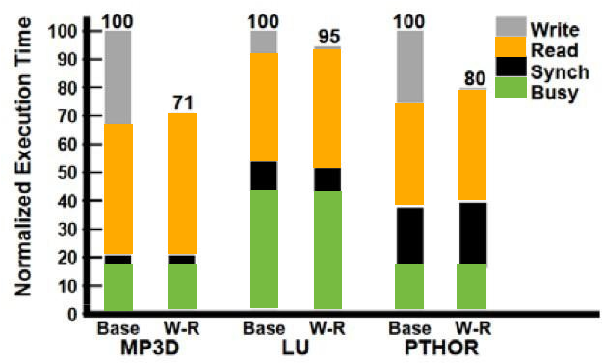
\includegraphics[width=.6\textwidth]{img/write-buffer-performance-1.pdf}
    \caption{Write Buffer Performance.}
    \label{fig: Write Buffer Performance}
\end{figure}

\begin{itemize}
    \item MP3D:
    \begin{itemize}
        \item Base (Sequential Consistency): 100 (normalized execution time)
        \item W-R (Write Buffer): 71 (normalized execution time)
        \item Performance Improvement: 29\% reduction in execution time.
    \end{itemize}

    \item LU:
    \begin{itemize}
        \item Base (Sequential Consistency): 100 (normalized execution time)
        \item W-R (Write Buffer): 95 (normalized execution time)
        \item Performance Improvement: 5\% reduction in execution time.
    \end{itemize}
    
    \item PTHOR:
    \begin{itemize}
        \item Base (Sequential Consistency): 100 (normalized execution time)
        \item W-R (Write Buffer): 80 (normalized execution time)
        \item Performance Improvement: 20\% reduction in execution time.
    \end{itemize}
\end{itemize}
These results indicate that the write buffer method can significantly improve performance in multiprocessor systems, especially in scenarios where write latency is a critical factor.
